\section{Enzhosor Ent Ino}\label{enzhosor-ent-ino}

Tags: NPC Alias: Il Satiro Creatore: Davide Ispirazione: Enzo Sorrentino
Luogo: Valtorria Razza: Elfo Classe: Bardo

\section{Enzhosor Ent Ino}\label{enzhosor-ent-ino-1}

\begin{center}\rule{0.5\linewidth}{0.5pt}\end{center}

\begin{figure}
\centering
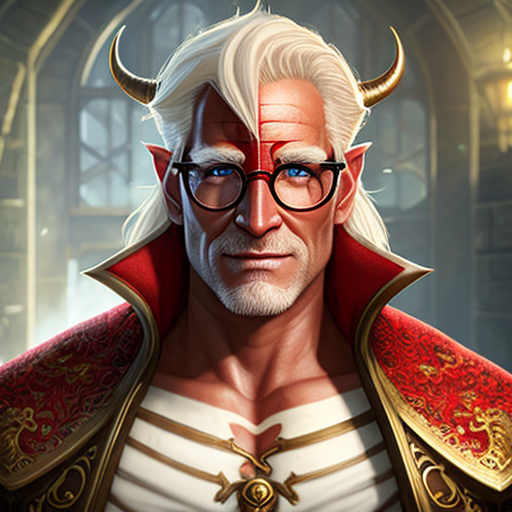
\includegraphics{a-male-tiefling-red-skin-and-blonde-hair-old-age-spectacles-.png}
\caption{a-male-tiefling-red-skin-and-blonde-hair-old-age-spectacles-.png}
\end{figure}

Informazioni Generali

Età: 62

Anno di nascita: 1961

Paese di nascita:

Razza: Mezzo tiefling

Professione: Sindaco

Alleati:

Nemesi:

Possedimenti importanti:

Conosciuto come: Il regista

\begin{center}\rule{0.5\linewidth}{0.5pt}\end{center}

\subsection{1. Descrizione Generale}\label{descrizione-generale}

\begin{center}\rule{0.5\linewidth}{0.5pt}\end{center}

\begin{figure}
\centering
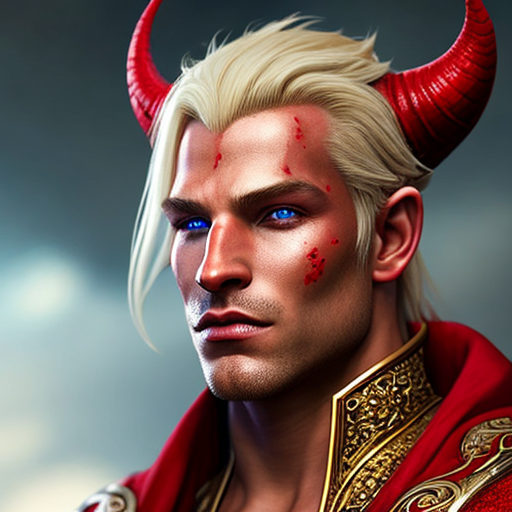
\includegraphics{a-male-tiefling-red-skin-and-blonde-hair-.png}
\caption{a-male-tiefling-red-skin-and-blonde-hair-.png}
\end{figure}

Enzhosor Ent Ino è un uomo di 62 anni, con capelli bianchi e crespi che
circondano la sua testa come una criniera. È un individuo dall'aspetto
fiero, con una statura media e una postura eretta. Indossa sempre abiti
eleganti e colorati, spesso arricchiti da gioielli e dettagli sontuosi.
I suoi occhi chiari, vivaci e intelligenti, riflettono la determinazione
che lo caratterizza.

\begin{quote}
``Satira!''
\end{quote}

\subsection{2. Biografia}\label{biografia}

\begin{center}\rule{0.5\linewidth}{0.5pt}\end{center}

Enzhosor è nato e cresciuto nella città di Valtorria, che un tempo era
un importante centro commerciale della regione. Sin da giovane, ha
dimostrato una grande passione per le arti drammaturgiche. Ha trascorso
la sua giovinezza viaggiando, portando il suo teatro tra le città e
villaggi di Valtara. Nonostante la sua forte autostima, le sue doti non
sono mai state apprezzate, ed in seguito ad uno spiacevole incidente, è
stato costretto a tornare a casa.

\subsubsection{2.1 Il fatale incidente}\label{il-fatale-incidente}

Durante uno dei suoi epici viaggi insieme alla sua compagnia teatrale,
Enzhosor si trovò improvvisamente costretto ad attraversare un antico
sentiero di montagna. La via, avvolta da un velo di mistero e gelo, si
stagliava sinistra e stretta, mentre il carro galleggiava sopra la
superficie ghiacciata. Il destriero di Enzhosor, aggraziato quanto un
unicorno, tentò invano di mantenere la presa, ma l'impeto
incontrollabile lo spinse verso l'abisso senza pietà.

Con un balzo acrobatico, Enzhosor si lanciò nell'aria, sfidando la
gravità e gli spiriti maligni che popolavano quei luoghi sconosciuti.
L'aura di un'antica profezia lo guidò verso un approdo sicuro,
salvandolo da un destino avverso. Tuttavia, il destino non ebbe pietà
per il resto della sua fida compagnia, imprigionata all'interno del
carro in fuga.

L'evento tragico, ancora oggi pesante nel cuore di Enzhosor, si rivelò
una scossa che sconvolse il suo spirito avventuroso. Decideva così di
porre fine alla sua vita come artista itinerante, abbandonando le strade
erranti per fare ritorno a Valtorria, un regno lontano, in cerca di
serenità e riscatto.

\subsection{3. Carriera}\label{carriera}

\begin{center}\rule{0.5\linewidth}{0.5pt}\end{center}

Dopo aver acquisito un'ampia conoscenza dell'animo umano, Enzhosor ha
deciso di stabilirsi a Valtorria e intraprendere una carriera politica.
Grazie alla sua capacità di negoziare e alle sue abilità di leadership,
è riuscito a diventare il sindaco della città. Da allora, ha concentrato
i suoi sforzi nell'ampliare il potere di Valtorria e aumentare la sua
influenza economica.

Enzhosor ha avviato molte iniziative per promuovere lo sviluppo
economico di Valtorria, come la creazione di nuovi mercati, l'attrazione
di investimenti e la promozione di alleanze commerciali con altre città.
Tuttavia, il suo desiderio di conquistare Azura per il controllo
completo dei commerci marittimi ha reso la sua politica più aggressiva e
ambiziosa.

\begin{figure}
\centering
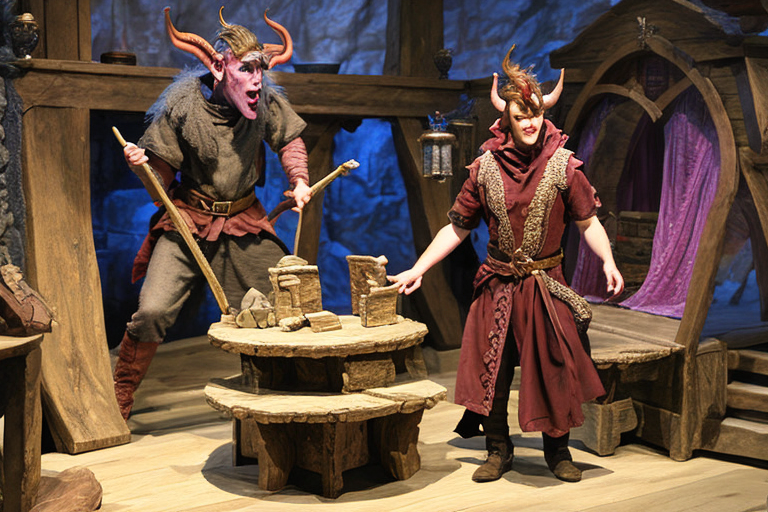
\includegraphics{a-fantasy-theatre-with-a-male-tiefling-playing--2.png}
\caption{a-fantasy-theatre-with-a-male-tiefling-playing--2.png}
\end{figure}

\subsection{4. Personalità}\label{personalituxe0}

\begin{center}\rule{0.5\linewidth}{0.5pt}\end{center}

Enzhosor è un uomo sicuro di sé, determinato e ambizioso. È convinto di
essere l'uomo più divertente del mondo, anche se spesso il suo senso
dell'umorismo è considerato piuttosto discutibile dagli altri. Adora
raccontare barzellette, inventarne di nuove e sorridere a se stesso
mentre le racconta, ma spesso le sue battute sono considerate forzate o
poco riuscite dagli altri.

Nonostante la sua personalità dominante e la sete di potere, Enzhosor è
anche un individuo intelligente e strategico. È abile nel riconoscere le
opportunità economiche e sa come sfruttarle a suo vantaggio. Tuttavia,
la sua brama di potere può portarlo a prendere decisioni poco etiche o a
ignorare il benessere degli altri.

In conclusione, Enzhosor Ent Ino è un sindaco ambizioso e carismatico,
determinato a espandere l'influenza di Valtorria. La sua personalità
carismatica e il suo senso dell'umorismo discutibile lo rendono un
personaggio interessante e controverso, pronto a sfidare gli altri per
raggiungere i suoi obiettivi.

\begin{quote}
``Enzo chiede a Kos: Hey Enzo, sei stato a Kos? Ma Kos? Kosa dici?
\ldots{} Satira''
\end{quote}

\subsection{A. Coinvolgimenti in eventi
recenti}\label{a.-coinvolgimenti-in-eventi-recenti}

\begin{center}\rule{0.5\linewidth}{0.5pt}\end{center}

\href{Untitled\%20Database\%20b540a0577b624713b0d8ac194cd482f5.csv}{Untitled
Database}

\subsection{B. Aggiornamenti}\label{b.-aggiornamenti}

\begin{center}\rule{0.5\linewidth}{0.5pt}\end{center}

\href{Untitled\%205bbba70bc8d14d398e68283ff572fd85.csv}{}
